\documentclass[10pt]{beamer}
%\documentclass[handout,10pt]{beamer}
\usepackage{my_style}
%%%%%%%%%%%%%%%%%%%%%%%%%%%%%%%%%%%%%%%%%%%%%%%%%%%%%%%%%%%%%%%%%%%%%%%%
%%%%%%%%%%%%%%%%%%%%%%%%%%%%%%%%%%%%%%%%%%%%%%%%%%%%%%%%%%%%%%%%%%%%%%%%

\title[Math/CS 375]{Lecture 05 - B}
\subtitle{\S 2.1 Counting Operations and Solving Special Systems}

\begin{document}
% -------------------------------------------------
\begin{frame}
  \titlepage
\end{frame}

% -------------------------------------------------
\begin{frame}{Goals}
We will answer these questions:\\[3mm]
\begin{itemize}
    \item How do you measure the cost of an algorithm?
    \item How and why do you benchmark code?
    \item How do you solve $Ax=b$ if $A$ is diagonal?
    \item How do you solve $Ax=b$ if $A$ is triangular? How expensive is it?
    \item How expensive is it to solve a banded system?
\end{itemize}
\end{frame}


%----------------------------------------------------
\sectionframe{Counting FLOPs}
%----------------------------------------------------

\begin{frame}{BLAS}
\textbf{Basic Linear Algebra Subprograms} (BLAS) interface introduced APIs for common linear algebra tasks:
  \begin{itemize}
  \item Level 1: vector operations (dot products, vector norms, etc) e.g.
    \[
    y \leftarrow \alpha x + y
    \]

  \item Level 2: matrix-vector operations, e.g.
    \[
    y \leftarrow \alpha A x +  B y
    \]

  \item Level 3: matrix-matrix operations, e.g.
    \[
    C \leftarrow \alpha A B +  \beta C
    \]
  \end{itemize}
BLAS is highly optimized. Almost everywhere software runs some version of BLAS under the hood.
\end{frame}

%%%%%%%%%%%%%%%%%%%%%%%%%%%%%%%%%%%%%%%%%%%%%%%%%%%%%%%%%%%%%%%%%%%%%%%%
\begin{frame}{FLOPs}
\define{FLOP}{
\begin{itemize}
    \item Adding, subtracting, multiplying, and dividing two floats is called a \textbf{floating point operation} (FLOP) 
    \item The plural will be abbreviated as FLOPs 
\end{itemize}
}

\begin{itemize}
    \item FLOP = unit of computational cost
    \item Example: count cost to evaluate polynomial $p(t)$
        
        \begin{align*}
            p(t) &= 3t^2 - 4t + 1\\
                 &= (3\times t \times t) - (4\times t) + 1
        \end{align*}
    \begin{itemize}
    \item 3 multiplications, 1 addition, 1 subtraction
    \item Evaluating $p(x)$ costs 5 FLOPs
    \end{itemize}
\end{itemize}
\end{frame}

%%%%%%%%%%%%%%%%%%%%%%%%%%%%%%%%%%%%%%%%%%%%%%%%%%%%%%%%%%%%%%%%%%%%%%%%
\begin{frame}[fragile]{Cost of Inner Product}{Level 1}
\begin{example}
    How many FLOPs are required to compute the inner product 
        $$ u^T v $$
    of vectors of length $n$? What is operation count in Big-O notation? 
\end{example}

\begin{itemize}
  \item The algorithm is
  \begin{align*}      
    u^T v &= u_1 v_1 + \dots + u_n v_n\\
          &= (u_1 \times v_1) + \dots + (u_n \times v_n)
  \end{align*}
  \item $n$ multiplies
  \item $n-1$ additions
  \item There is exactly $2n-1$ FLOPs 
  \item Cost is $\mO(n)$ FLOPs
\end{itemize}
\end{frame}

%%%%%%%%%%%%%%%%%%%%%%%%%%%%%%%%%%%%%%%%%%%%%%%%%%%%%%%%%%%%%%%%%%%%%%%%

\begin{frame}[fragile]{Cost of Matrix-Vector Multiplication}{Level 2}
\begin{example}
    How many FLOPs are required to compute the matrix-vector product
        $$ v = Au$$
    in Big-O notation?
\end{example}

\begin{itemize}
    \item The algorithm is
\begin{lstlisting}[mathescape]
for $i=1,\dots,n$
   for $j=1,\dots,n$
      v(i) $\leftarrow$  v(i) +  a(i,j)*u(j)  % executed n^2 times
   end
end
\end{lstlisting}
  \item $n^2$ multiplications and  $n^2$ additions
  \item Cost is $\mO(n^2)$ FLOPs
\end{itemize}
\end{frame}
%%%%%%%%%%%%%%%%%%%%%%%%%%%%%%%%%%%%%%%%%%%%%%%%%%%%%%%%%%%%%%%%%%%%%%%%
\begin{frame}[fragile]{Cost of Matrix-Matrix Multiplication}{Level 3}
\begin{example}
    How many FLOPs are required to compute the matrix-matrix product 
        $$C = AB$$
    in Big-O notation? (Assume we are using standard algorithm)
\end{example}
\begin{itemize}
\item The algorithm is
\begin{lstlisting}[mathescape]
for $j=1,\dots,n$
   for $i=1,\dots,n$
      for $k=1,\dots,n$
         C(k,j) $\leftarrow$ C(k,j) + A(k,i)*B(i,j) % n^3 times
      end
   end
end
\end{lstlisting}
  \item $n^3$ multiplications and  $n^3$ additions
  \item Cost is $\mO(n^3)$ FLOPs
\end{itemize}
\end{frame}
%%%%%%%%%%%%%%%%%%%%%%%%%%%%%%%%%%%%%%%%%%%%%%%%%%%%%%%%%%%%%
\begin{frame}[shrink]{The Order of Computation Matters}

\begin{example}
Let $A,B\in\mathbb{R}^{n\times n}$ and
$x\in\mathbb{R}^n$. Compare the cost of evaluating
\[
    (AB)x
    \qquad \text{and} \qquad
    A(Bx).
\]
Assume dense matrices and standard multiplication.
\end{example}

\begin{itemize}
    \item<2-> Compute $(AB)x$:
    \begin{itemize}
        \item Form $C=AB$: $\mO(n^3)$ FLOPs.
        \item Compute $Cx$: $\mO(n^2)$ FLOPs.
        \item Total: $\boxed{\mO(n^3)}$.
    \end{itemize}

    \vfill

    \item<3-> Compute $A(Bx)$:
    \begin{itemize}
        \item Form $y=Bx$: $\mO(n^2)$ FLOPs.
        \item Compute $Ay$: $\mO(n^2)$ FLOPs.
        \item Total: $\boxed{\mO(n^2)}$.
    \end{itemize}
\end{itemize}

\onslide<4->{
\keyidea{
The expressions are equal in exact arithmetic,
but their computational costs are very different.
}
}

\end{frame}


%%%%%%%%%%%%%%%%%%%%%%%%%%%%%%%%%%%
\sectionframe{Benchmarking Code}
%%%%%%%%%%%%%%%%%%%%%%%%%%%%%%%%%%%
\begin{frame}{Why do we time our code?}

    \textbf{Benchmarking code} refers to calculating the wallclock runtime of your code from beginning to end.\\[5mm]

    Reasons:\\[3mm]
    \begin{itemize}
        \item To identify bottlenecks in your program.
        \item To compare different algorithms or implementations.
        \item To predict how your algorithm scales for large input size.
    \end{itemize}
\end{frame}

%%%%%%%%%%%%%%%%%%%%%%%%%%%%%%%%%%%%%%%%%%%%%%%%%%%%%%%%%%%%%%%%%%%%%%%%

\begin{frame}[fragile]{Tic-Toc}
    \begin{itemize}
        \item Matlab provides \texttt{tic} and \texttt{toc} commands to measure elapsed time.
        \item Basic usage:
\begin{lstlisting}[mathescape]
tic
% Code to measure
toc
\end{lstlisting}
        \item Output: Elapsed time in seconds.
    \end{itemize}

\vspace{3mm}

\textbf{Example:}
\begin{lstlisting}[mathescape]
A = rand(1000,1000);
x = rand(1000,1);
tic
y = A*x;
elapsed_time = toc;
fprintf('Elapsed time: %f seconds\n', elapsed_time);
\end{lstlisting}
\end{frame}



%%%%%%%%%%%%%%%%%%%%%%%%%%%%%%%%%%%%%%%%%%%%%%%%%%%%%%%%%%%%%%%%%%%%%%%%

\begin{frame}[fragile]{Timing $u'v$ in Matlab}
\begin{lstlisting}
n = 1000; % size of vectors
u = rand(n,1);
v = rand(n,1);

tic % begin clock 

for j = 1 : 10 % do ten trials 
    ip = u'*v;
end

avg_time = toc/10; % average result
\end{lstlisting}

\begin{itemize}
    \item The inner product  $u'v$ is computed 10 times
    \item Divide total runtime by 10
    \item Repeat this for $n=10^5, 10^6, 10^7, 10^8$
\end{itemize}
\end{frame}
%%%%%%%%%%%%%%%%%%%%%%%%%%%%%%%%%%%%%%%%%%%%%%%%%%%%%%%%%%%%%%%%%%%%%%%%
\begin{frame}[fragile]{Result Over Ten Trials}

\begin{center}
  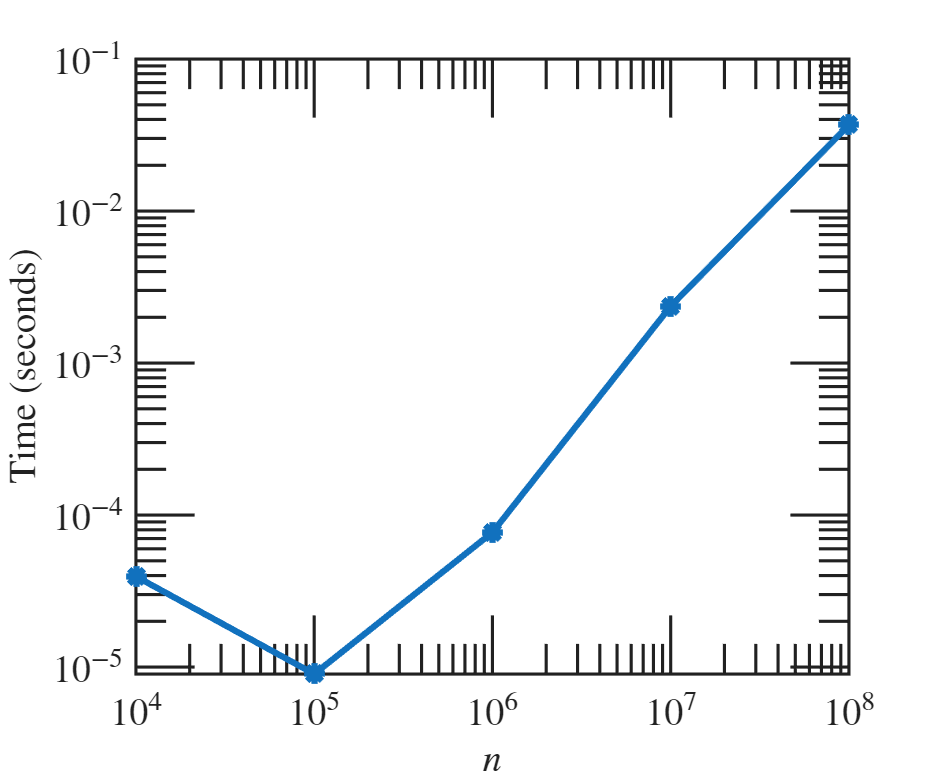
\includegraphics[height=5.8cm]{./figs/runtime_vecvec_n10.png}
\end{center}
   \vspace{-7pt}
\begin{itemize}
    \item Plot runtime on log-log scale 
    \item Runtime plots rarely look perfect due to \textbf{randomness}
    \item Ten trials is \textit{not enough!}
\end{itemize}
\end{frame}



%%%%%%%%%%%%%%%%%%%%%%%%%%%%%%%%%%%%%%%%%%%%%%%%%%%%%%%%%%%%%%%%%%%%%%%%
\begin{frame}[fragile]{Counting Ticks}
\begin{center}
  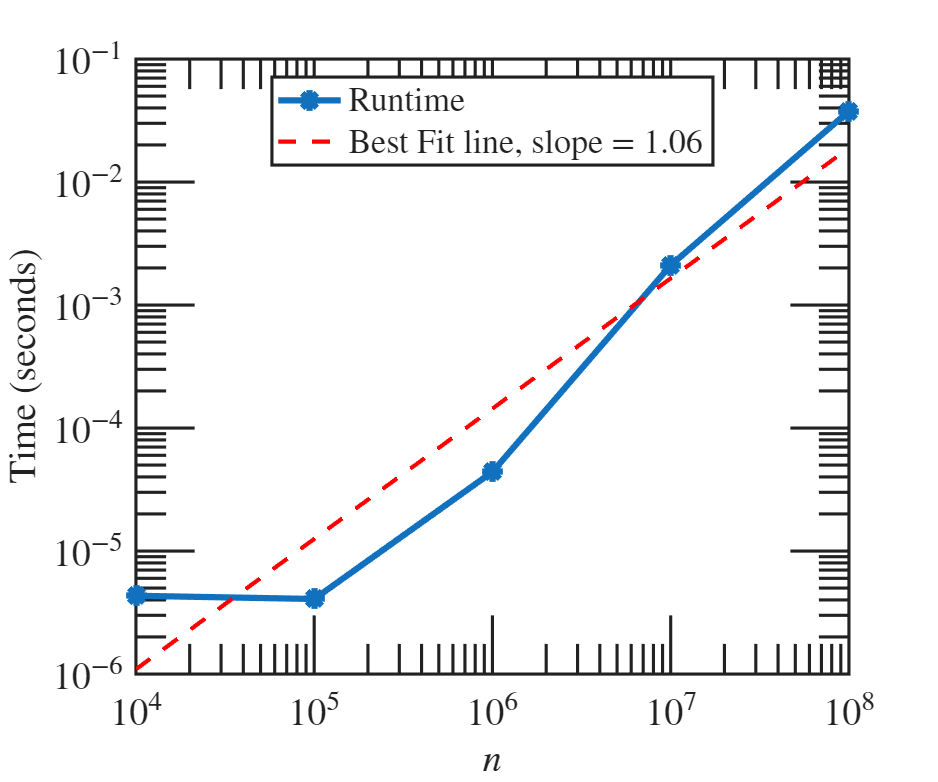
\includegraphics[height=5cm]{./figs/runtime_vecvec_line.png}
\end{center}

\begin{itemize}
    \item Calculate slope on log-log plot by counting tick marks
    \item Counting by orders of 10 
        \begin{align*}
            \Delta x = 4\\
            \Delta y = 4
        \end{align*}
    \item Slope $m = \frac{\Delta y}{\Delta x}=1$ which means cost is $\mO(n)$
\end{itemize}
\end{frame}

%%%%%%%%%%%%%%%%%%%%%%%%%%%%%%%%%%%%%%%%%%%%%%%%%%%%%%%%%%%%%%%%%%%%%%%%

\begin{frame}{Benchmarking Tips}

    \begin{block}{Strongly Reccomend}
        
    \begin{itemize}
        \item Warm-up runs: Run your code a few times before measuring to ensure consistent performance.\\[3mm]
        \item System noise: Close background processes that can interfere with timing.\\[3mm]
        \item Multiple trials: Always average results over several runs.  \\[3mm]
    \end{itemize}
    \end{block}

    \vspace{3mm}
    \begin{block}{Optional}
    \begin{itemize}
        \item Vectorize your code: Matlab favors vectorized code over for-loops.\\[3mm]
        \item Profiling: Use Matlab's \texttt{profile} command for detailed performance analysis. It is useful for spotting bottle necks.\\[3mm]
        \item Alerts: You can program Matlab to play a sound or send an email when it is finished.
    \end{itemize}
    \end{block}
\end{frame}




%%%%%%%%%%%%%%%%%%%%%%%%%%%%%%%%%%%
\sectionframe{Solving Special Systems}
%%%%%%%%%%%%%%%%%%%%%%%%%%%%%%%%%%

\begin{frame}{Cost to Solve $Ax=b$}

\begin{itemize}
    \item Suppose $A\in\mathbb{R}^{n\times n}$
        \vfill 
    \item How many FLOPs does it cost to solve 
    $$Ax=b?$$
        \vfill 
    \item Let's begin by considering special matrices
\end{itemize}
    
\end{frame}

\begin{frame}{Special Matrices}
\begin{itemize}
    \item \textbf{Diagonal}
    \[
    \begin{bmatrix}
    \bullet & 0 & 0 & 0 \\
    0 & \bullet & 0 & 0 \\
    0 & 0 & \bullet & 0 \\
    0 & 0 & 0 & \bullet
    \end{bmatrix}
    \]

    \item \textbf{Triangular}
    \[
    \begin{bmatrix}
    \bullet & \bullet & \bullet & \bullet \\
    0 & \bullet & \bullet & \bullet \\
    0 & 0 & \bullet & \bullet \\
    0 & 0 & 0 & \bullet
    \end{bmatrix}
    % \quad \text{(Upper Triangular)} \quad
    % \begin{bmatrix}
    % \bullet & 0 & 0 & 0 \\
    % \bullet & \bullet & 0 & 0 \\
    % \bullet & \bullet & \bullet & 0 \\
    % \bullet & \bullet & \bullet & \bullet
    % \end{bmatrix}
    % \quad \text{(Lower Triangular)}
    \]

    \item \textbf{Banded}
    \[
    \begin{bmatrix}
    \bullet & \bullet & 0 & 0 \\
    \bullet & \bullet & \bullet & 0 \\
    0 & \bullet & \bullet & \bullet \\
    0 & 0 & \bullet & \bullet
    \end{bmatrix}
    \]
\end{itemize}

\end{frame}


%%%%%%%%%%%%%%%%%%%%%%%%%%%%%%%%%%%%%%%%%%%%%%%%%%%%%%%%%%%%%%%%%%%%%%%%
\begin{frame}{Solving Diagonal Systems}

\onslide<1->{

\define{Diagonal Matrix}{
A matrix $A$ is \textbf{diagonal} if $a_{ij}=0$ for all $i\neq j$. 
}
Suppose you wish to solve $Ax=b$, where
\begin{equation*}
    A = \begin{bmatrix}2 & 0 & 0\\ 0 & 3 & 0\\ 0 & 0 & 5 \end{bmatrix}
    \ \ \ \ \ \ \
    b = \left[\negthickspace\begin{array}{r} -1 \\ 6 \\ -15 \end{array}\negthickspace\right]
\end{equation*}
}
\onslide<2->{
Writing out the system
\begin{equation*}
    \begin{array}{ccccr}
      2x_1 &       &        &= &  -1  \\
          & 3 x_2 &        &= &   6  \\
          &       &  5 x_3 &= & -15
    \end{array}
\end{equation*}
}
\onslide<3->{
The solution is
\begin{align*}
    x_1 &= -\frac{1}{2}  &
    x_2 &= \frac{6}{3}=2 &
    x_3 &= \frac{-15}{5} = -3
\end{align*}
}

\end{frame}

%%%%%%%%%%%%%%%%%%%%%%%%%%%%%%%%%%%%%%%%%%%%%%%%%%%%%%%%%%%%%%%%%%%%%%%%
\begin{frame}[fragile]{Diagonal Solve}

\begin{lstlisting}[mathescape,caption=Diagonal System Solution,label=algo:diagSolv]
given $A$, $b$              
for $i=1\ldots n$           
   $x_i = b_i/a_{ii}$       
end                         
\end{lstlisting}

\method{Diagonal Solve}{Diagonal matrix $A$, right hand side $b$}{
Solution to $Ax=b$
}{
Take advantage of the structure of $A$
}

\end{frame}
%%%%%%%%%%%%%%%%%%%%%%%%%%%%%%%%%%%%%%%%%%%%%%%%%%%%%%%%%%%%%%%%%%%%%%%%
\begin{frame}[fragile]{Operation Count}

{\question{
How expensive is it to solve $Ax=b$ if $A$ is diagonal?
}}

\begin{lstlisting}[mathescape]       
for $i=1\ldots n$           
   $x_i = b_i/a_{i,i}$  % executed n times
end                         
\end{lstlisting}

\keyidea{
\begin{itemize}
    \item Solving $Ax=b$ costs only $\mO(n)$ FLOPs
    \item $\mO(n)$ cost is considered to be \textit{very fast}
\end{itemize}
}

\end{frame}


%%%%%%%%%%%%%%%%%%%%%%%%%%%%%%%%%%%%%%%%%%%%%%%%%%%%%%%%%%%%%%%%%%%%%%%%
\sectionframe{Triangular System}
%%%%%%%%%%%%%%%%%%%%%%%%%%%%%%%%%%%%%%%%%%%%%%%%%%%%%%%%%%%%%%%%%%%%%%%%
\begin{frame}{Triangular Systems}

The generic lower and upper triangular matrices are
\begin{equation*}
    L = \begin{bmatrix} l_{11} &   0    & \cdots &   0    \\
                        l_{21} & l_{22} &        &   0    \\
                        \vdots &        & \ddots & \vdots \\
                        l_{n1} &        & \cdots & l_{nn} \\
        \end{bmatrix}
\end{equation*}
and
\begin{equation*}
    U = \begin{bmatrix} u_{11} & u_{12} & \cdots & u_{1n} \\
                           0   & u_{22} &        & u_{2n}  \\
                        \vdots &        & \ddots & \vdots \\
                           0   &        & \cdots & u_{nn} \\
        \end{bmatrix}
\end{equation*}

The triangular systems
\begin{equation*}
    Ly = b \ \ \ \ \ \ \ \ \ Ux = c
\end{equation*}
are easily solved by \textbf{forward substitution} and
\textbf{backward substitution}, respectively

\end{frame}
%%%%%%%%%%%%%%%%%%%%%%%%%%%%%%%%%%%%%%%%%%%%%%%%%%%%%%%%%%%%%%%%%%%%%%%%
\begin{frame}{Solving Triangular Systems}{Part 1}

\onslide<1->{
\begin{example}
Solve $Ax=b$ where 
\begin{equation*}
    A = \left[\negthickspace\begin{array}{rrr} -2 & 1 & 2 \\ 0 & 3 & -2 \\ 0 & 0 & 4\end{array}\negthickspace\right]
    \ \ \ \ \ \ \
    b = \left[\negthickspace\begin{array}{r} 9 \\ -1 \\ 8 \end{array}\negthickspace\right]
\end{equation*}
and count the total number of FLOPs.
\end{example}
}

\begin{itemize}
    \item<2-> First, write out the system
\begin{equation*}
    \begin{array}{rcrcrcr}
      -2 x_1 & + &   x_2  & + &  2x_3 &= &  9  \\
             &   &  3x_2  & + & -2x_3 &= & -1  \\
             &   &        &   &  4x_3 &= &  8  \\
    \end{array}
\end{equation*}

    \item<3-> Solve for $x_3$ first. 
\begin{align*}
      x_3 &= \frac{8}{4} = 2 \quad \text{\color{red}one FLOP}
\end{align*}

\end{itemize}
\end{frame}
%%%%%%%%%%%%%%%%%%%%%%%%%%%%%%%%%%%%%%%%%%%%%%%%%%%%%%%%%%%%%%%%%%%%%%%%
\begin{frame}{Solving Triangular Systems}{Part 2}
\begin{equation*}
    \begin{array}{rcrcrcr}
      -2 x_1 & + &   x_2  & + &  2x_3 &= &  9  \\
             &   &  3x_2  & + & -2x_3 &= & -1  \\
             &   &        &   &  4x_3 &= &  8  \\
    \end{array}
\end{equation*}

\begin{itemize}
    \item We have $x_3$  
    $$
          x_3 = \frac{8}{4} = 2 \quad \text{{\color{red}one FLOP}}
    $$
    \item<2-> Next, we solve for $x_2$
    $$
    x_2 = \frac{-1+2\times x_3}{3}   =1
    \quad \text{\color{red}three FLOPs}
    $$
    \item<3-> Finally, we solve for $x_1$
    $$
x_1 = \frac{9-1\times x_2-2\times x_3}{-2}
    =-2
    \quad \text{\color{red}five FLOPs}
    $$
    \item<4-> Total: 1+3+5 = {\color{red}9 FLOPs}
\end{itemize}
\end{frame}
%%%%%%%%%%%%%%%%%%%%%%%%%%%%%%%%%%%%%%%%%%%%%%%%%%%%%%%%%%%%%%%%%%%%%%%%
\begin{frame}[fragile]{Backward Substitution}
This algorithm is called \textbf{backward substitution} 
\begin{lstlisting}[mathescape,label=algo:backsub]
given $U$ (upper $\bigtriangleup$), $b$               
$x_n = b_n/u_{nn}$           
for $i=n-1\ldots 1$ % loop backwards         
    $s = b_i$                  
    for $j = i+1\ldots n$    
        $s = s - u_{i,j}x_j$   
    end                      
    $x_i = s/u_{i,i}$          
end                          
\end{lstlisting}

\method{Backward substitution}
{Upper triangular $U$, right-hand side $b$}
{Solution to $Ux=b$}
{Solve backwards $x_n$, $x_{n-1}$, $\ldots$, $x_1$ for max efficiency}
\end{frame}
%%%%%%%%%%%%%%%%%%%%%%%%%%%%%%%%%%%%%%%%%%%%%%%%%%%%%%%%%%%%%%%%%%%%%%%%
\begin{frame}{Lower Triangular System}
\begin{itemize}
    \item Consider this example
    \begin{equation*}
        A = \left[\negthickspace\begin{array}{rrr} 
            4 & 0 & 0 \\
            -2 & 3 & 0 \\ 
            -2 & 1 & 2 \\ 
            \end{array}\negthickspace\right]
        \ \ \ \ \ \ \
        b = \left[\negthickspace\begin{array}{r} 
        8 \\
        -1 \\
        9 \\
        \end{array}\negthickspace\right]
    \end{equation*}

\item When written out, the simplest way to proceed becomes obvious
\begin{equation*}
    \begin{array}{rcrcrcr}
         4x_1    &   &        &   &   &= &  8  \\
         -2x_1    &  + &  3x_2  &  &  &= & -1  \\
      -2 x_1 & + &   x_2  & + &  2x_3 &= &  9  \\
    \end{array}
\end{equation*}

\item Solve in forward order 
\begin{align*}
      x_1 &= \frac{8}{4} = 2
    & x_2 &= \frac{1}{3} \left( -1 + 2 x_3 \right) = \frac{3}{3} = 1
    \\
    & &  x_3 &= \frac{9+2x_1-x_2}{2}=6.
\end{align*}

\item The idea is the same as \textbf{backward substitution} but in reverse

\end{itemize}
\end{frame}

%%%%%%%%%%%%%%%%%%%%%%%%%%%%%%%%%%%%%%%%%%%%%%%%%%%%%%%%%%%%%%%%%%%%%%%%

\begin{frame}[fragile]{Forward Substitution}

This algorithm is called \textbf{forward substitution} 
\begin{lstlisting}[mathescape,caption=,label=algo:forsub]
given $L$ (lower $\bigtriangleup$), $b$               
$x_1 = b_1/\ell_{11}$           
for $i=2\ldots n$  % loop forward        
    $s = b_i$                 
    for $j = 1\ldots i-1$    
        $s = s - \ell_{i,j}x_j$   
    end                      
    $x_i = s/\ell_{i,i}$          
end                          
\end{lstlisting}

\method{Forward substitution}
{Lower triangular $L$, right-hand side $b$}
{Solution to $Lx=b$}
{Solve in forward sequence $x_1$,$\ldots$,$x_n$ for max efficiency}

Forward and backward substitution are \textbf{triangular solves}.

\end{frame}

%%%%%%%%%%%%%%%%%%%%%%%%%%%%%%%%%%%%%%%%%%%%%%%%%%%%%%%%%%%%%%%%%

\begin{frame}{Operation-Counting Formula}

{
\question{How expensive is to perform triangular solves for a matrix of size $n$?}
}


Here is a useful formula
\begin{block}{Sum of the First $n$ Integers}
     $$\sum_{j=1}^{n} j =  \frac{ n(n+1)}{2} = \mO(n^2)$$
\end{block}

\textbf{Proof:}
Let $S=1+2+\cdots+n$. Then
\[
\begin{aligned}
    S &= 1+2+\cdots+n,\\
    S &= n+(n-1)+\cdots+1.
\end{aligned}
\]
Adding corresponding terms gives
\[
    2S=n(n+1),
    \qquad
    S=\frac{n(n+1)}{2}.
\]
\end{frame}

%%%%%%%%%%%%%%%%%%%%%%%%%%%%%%%%%%%%%%%%%%%%%%%%%%%%%%%%%%%%%%%%%%%%%%%%
\begin{frame}[shrink]{Operation Count for $n\times n$}

Suppose $A \in \mathbb{R}^{n \times n}$ is lower triangular. Forward substitution will cost:\\[2mm]
  \begin{itemize}
    \item row 1: 1 div = 1 FLOP
    \item row 2: 1 mult, 1 add, 1 div =  3 FLOPs
    \item row 3: 2 mult, 2 add, 1 div = 5 FLOPs
    \item row 4: 3 mult, 3 add, 1 div = 7 FLOPs
    \item  $\quad\vdots$
\item row $j$: $(j-1)$ multiplications,
$(j-1)$ subtractions, and 1 division:
\[
    2(j-1)+1=2j-1 \text{ FLOPs}.
\]
  \end{itemize}

\begin{block}{Total FLOPs}
\[
    \sum_{j=1}^n (2j-1)
    =
    2\frac{n(n+1)}{2}-n
    =
    \boxed{n^2}.
\]
\end{block}

\keyidea{
Forward and backward substitution each cost
$\mO(n^2)$ FLOPs for a dense triangular system.
}

\end{frame}


%%%%%%%%%%%%%%%%%%%%%%%%%%%%%%%%%%%%%%%%%%%%%%%%%%%%%%%%%%%%%%%%%%%%%%%%
\sectionframe{Banded Systems}
%%%%%%%%%%%%%%%%%%%%%%%%%%%%%%%%%%%%%%%%%%%%%%%%%%%%%%%%%%%%%%%%%%%%%%%%

\begin{frame}[shrink]{Example: Upper Bidiagonal System}{Part 1}
\begin{example}
Solve the $4 \times 4$ \textbf{upper bidiagonal} system
\[
B =
\begin{bmatrix}
2 & 1 & 0 & 0 \\
0 & 3 & 4 & 0 \\
0 & 0 & 5 & 2 \\
0 & 0 & 0 & 6
\end{bmatrix}, \quad
b =
\begin{bmatrix}
5 \\ 19 \\ 26 \\ 18
\end{bmatrix}.
\]
For a general $n\times n$, what is the operation count?
\end{example}

We use back substitution:
\begin{align*}
x_4 &= \frac{b_4}{B_{44}} = \frac{18}{6} = 3\quad &\text{1 FLOP} \\
x_3 &= \frac{b_3 - B_{34} x_4}{B_{33}} = \frac{26 - 2\cdot 3}{5} = \frac{20}{5} =4\quad &\text{3 FLOPs} \\
x_2 &= \frac{b_2 - B_{23} x_3}{B_{22}} = \frac{19 - 4 \cdot 4}{3} = \frac{19 -16}{3}  = 1\quad &\text{3 FLOPs} \\
x_1
&= \frac{b_1-B_{12}x_2}{B_{11}}
 = \frac{5-1\cdot1}{2}
 = \frac{4}{2}
 = 2
\quad &\text{3 FLOPs}
\end{align*}
\end{frame}

%%%%%%%%%%%%%%%%%%%%%%%%%%%%%%%%%%%%%%%%%%%%%%%%%%%%%%%%%%%%
\begin{frame}[shrink]{Example: Upper Bidiagonal System}{Part 2}
\begin{itemize}
    \item Each step of back substitution (except the first) uses:
    \begin{itemize}
        \item 1 multiply
        \item 1 subtract
        \item 1 divide\\[3mm]
    \end{itemize}
    
    \item Total number of FLOPs $= 1 + 3 + 3 + 3 = 10 $\\[3mm]

\item For an $n\times n$ upper bidiagonal system,
\[
    \text{Total FLOPs}=1+3(n-1)=3n-2=\mO(n).
\]
\end{itemize}
\medskip

\keyidea{It is often easier to count operations by rows. For a bidiagonal, the cost to solve is only $\mO(n)$ which is very fast!}

\end{frame}

%%%%%%%%%%%%%%%%%%%%%%%%%%%%%%%%%%%%%%%%%%%%%%%%%%%%%%%

\begin{frame}{Tridiagonal}
\define{Tridiagonal Matrix}{

A \textbf{tridiagonal} matrix has the form
\begin{equation*}
\begin{bmatrix}
d_1 & c_1 &       &         &       &       &          &    \\
a_1 & d_2 & c_2   &         &       &       &          &    \\
     & \ddots & \ddots   & \ddots &       &          &    \\
     &       & a_{i-1} & d_i   & c_{i} &          &    \\
     &       &         & \ddots & \ddots & \ddots    &    \\
     &       &         &       & \ddots & \ddots    & c_{n-1}   \\
     &       &         &       &       & a_{n-1}  & d_n   \\
\end{bmatrix}.
\end{equation*}
The empty entries denote zeros.
}
\begin{itemize}
  \item Many of the entries are zeros 
  \item We can utilize \textit{row operations} to simplify the system
\end{itemize}
\end{frame}
%%%%%%%%%%%%%%%%%%%%%%%%%%%%%%%%%%%%%
\begin{frame}{Review: Elementary Row Operations}

The following operations preserve the solution set of $Ax=b$:

\begin{itemize}
    \item Swap two rows:
    \[
        R_i \leftrightarrow R_j.
    \]

    \item Multiply a row by a nonzero scalar:
    \[
        R_i \leftarrow cR_i, \qquad c\neq0.
    \]

    \item Add a multiple of another row:
    \[
        R_i \leftarrow R_i+cR_j, \qquad i\neq j.
    \]
\end{itemize}



\end{frame}
%%%%%%%%%%%%%%%%%%%%%%%%%%%%%%%%%%%%%%
\begin{frame}{Tridiagonal Elimination}{Example}

\begin{example}
Use elimination to turn this system into an
upper bidiagonal system:
\[
\left[
\begin{array}{rrr|r}
    2&1&0&4\\
    4&5&1&17\\
    0&6&4&24
\end{array}
\right].
\]
\end{example}

\begin{itemize}
    \item<2-> Apply $R_2\leftarrow R_2-2R_1$:
    \[
    \left[
    \begin{array}{rrr|r}
        2&1&0&4\\
        0&3&1&9\\
        0&6&4&24
    \end{array}
    \right].
    \]

    \item<3-> Apply $R_3\leftarrow R_3-2R_2$:
    \[
    \left[
    \begin{array}{rrr|r}
        2&1&0&4\\
        0&3&1&9\\
        0&0&2&6
    \end{array}
    \right].
    \]

    \item<4-> The resulting system is upper bidiagonal
    and can be solved by backward substitution.
\end{itemize}

\end{frame}
%%%%%%%%%%%%%%%%%%%%%%%%%%%%%%%%%%%%%%%%%%%%%%%%%%%%%%%%%%%%%%%%%%%%%%%%
\begin{frame}{Tridiagonal}
\begin{equation*}
\begin{bmatrix}
d_1 & c_1 &       &         &       &       &          &    \\
a_1 & d_2 & c_2   &         &       &       &          &    \\
& a_2 & d_3   & c_3     &       &       &          &    \\
&     & \ddots & \ddots   & \ddots &       &          &    \\
&     &       & a_{i-1} & d_i   & c_{i} &          &    \\
&     &       &         & \ddots & \ddots & \ddots    &    \\
&     &       &         &       & \ddots & \ddots    & c_{n-1}   \\
&     &       &         &       &       & a_{n-1}  & d_n   \\
\end{bmatrix}
\end{equation*}
Start forward elimination (without pivoting)
\begin{enumerate}
  \item subtract $a_1/d_1$ times row 1 from row 2
  \item this eliminates $a_1$, changes $d_2$ and does not touch $c_2$
  \item continuing:
\begin{equation*}
  d_{i} = d_{i} - \left(\frac{a_{i-1}}{d_{i-1}} c_{i-1}\right)
\end{equation*}
for $i=2\dots n$
\end{enumerate}
\end{frame}
%%%%%%%%%%%%%%%%%%%%%%%%%%%%%%%%%%%%%%%%%%%%%%%%%%%%%%%%%%%%%%%%%%%%%%%%
%%%%%%%%%%%%%%%%%%%%%%%%%%%%%%%%%%%%%%%%%%%%%%%%%%%%%%%%%%%%%%%%%%%%%%%%
\begin{frame}{Tridiagonal}
\begin{equation*}
  \begin{bmatrix}
{d}_1 & c_1 &       &         &       &       &          &    \\
 & {\tilde{d}}_2 & c_2   &         &       &       &          &    \\
    & & {\tilde{d}}_3   & c_3     &       &       &          &    \\
    &     &  & \ddots   & \ddots &       &          &    \\
    &     &       &  & {\tilde{d}}_i   & c_{i} &          &    \\
    &     &       &         & & \ddots & \ddots    &    \\
    &     &       &         & & & \ddots    &  c_{n-1}  \\
    &     &       &         &       &       & & {\tilde{d}}_n   \\
  \end{bmatrix}
\end{equation*}
This leaves an upper triangular (2-band).  With back substitution:
\begin{enumerate}
  \item $x_n = {\tilde{b}}_n/{\tilde{d}}_n$
  \item $x_{i} = (1/{\tilde{d}}_{i})({\tilde{b}}_{i} - c_{i}x_{i+1})$ for $i = n-1$ to 1
\end{enumerate}
\end{frame}

%%%%%%%%%%%%%%%%%%%%%%%%%%%%%%%%%%%%%%%%%%%%%%%%%%%%%%%%%%%%
\begin{frame}[fragile]{Tridiagonal Algorithm}
\begin{lstlisting}[mathescape,caption=Thomas Algorithm]
input: $n, a, d, c, b$
for $i=2$ to $n$
   $xmult = a_{i-1}/d_{i-1}$
   $d_i = d_i - xmult \cdot c_{i-1}$
   $b_i = b_i - xmult \cdot b_{i-1}$
end
$x_{n} = b_{n}/d_{n}$
for $i=n-1$ down to $1$
   $x_{i} = (b_{i} - c_{i} x_{i+1})/d_{i}$
end
\end{lstlisting}

\vspace{4mm}

The algorithm to solve a tridiagonal system is also $\mO(n)$ - \emph{very fast!}

\end{frame}

%%%%%%%%%%%%%%%%%%%%%%%%%%%%%%%%%%%%%%%%%%%%%%%%%%%%%%%%%%%%
%%%%%%%%%%%%%%%%%%%%%%%%%%%%%%%%%%%%%%%%%%%%%%%%%%%%%%%%%%%%
% \begin{frame}{Cost of the Tridiagonal Solve}

% \question{
% How many FLOPs does the Thomas algorithm require
% for an $n\times n$ system?
% }

% \begin{itemize}
%     \item<2-> Each forward-elimination step computes
%     \[
%     \begin{aligned}
%         q_i &= a_{i-1}/d_{i-1}
%             && \text{1 FLOP},\\
%         d_i &\leftarrow d_i-q_i c_{i-1}
%             && \text{2 FLOPs},\\
%         b_i &\leftarrow b_i-q_i b_{i-1}
%             && \text{2 FLOPs}.
%     \end{aligned}
%     \]
%     There are $n-1$ steps, giving $5(n-1)$ FLOPs.

%     \vfill

%     \item<3-> The resulting system is upper bidiagonal.
%     Backward substitution costs
%     \[
%         1+3(n-1)=3n-2 \text{ FLOPs}.
%     \]

%     \item<4-> The total cost is
%     \[
%         \boxed{5(n-1)+(3n-2)=8n-7=\mO(n).}
%     \]
% \end{itemize}

% \end{frame}
% \begin{frame}{General Banded System}
% \define{Banded System}{
% A $n\times n$ matrix is \textbf{banded} if it contain zero elements $a_{ij}=0$ for $|i-j|\geq k$.
% }

% \begin{itemize}
%   \item Elements $a_{ij}$ with $i=j$ corresponds to the diagonal
%   \item The integer $|i-j|$ corresponds to distance from diagonal
%   \item \textbf{Bandwidth} $m = 2k-1$ = maximum width of nonzero elements  
% \begin{center}
% \pgfimage[width=0.4\textwidth]{./figs/band5} 
% \end{center}
%   \item Consider distance $k=3$ 
%   \item The bandwidth is $m=2(3)-1=5$
% \end{itemize}

% \end{frame}
%%%%%%%%%%%%%%%%%%%%%%%%%%%%%%%%%%%%%%%%%%%%%%%%%%%%%%%%%%%%%%%%%%%%%%%%

\begin{frame}{$m$-band Cost}
\begin{tabular}{c c c}
\pgfimage[width=0.3\textwidth]{./figs/band5} & 
\pgfimage[width=0.3\textwidth]{./figs/band11} & 
\pgfimage[width=0.3\textwidth]{./figs/band11b}\\
$m=5$ & $m=11$ & $m=11$\\
\end{tabular}

\begin{block}{Cost for banded systems}
\begin{itemize}
    \item  If $A$ has bandwidth $m$, then solving $Ax=b$ cost $\mO(m^2n)$ FLOPs.\\
    \item This information is not in your textbook.
\end{itemize}
\end{block}
\end{frame}

%%%%%%%%%%%%%%%%%%%%%%%%%%%%

\begin{frame}{Summary of Costs}

\begin{block}{Operations}
\begin{itemize}
    \item inner product $u^Tv$: $\mO(n)$
    \item matrix-vector product $Ax$: $\mO(n^2)$
    \item matrix-matrix product $AB$: $\mO(n^3)$
\end{itemize}
\end{block}

\begin{block}{Solvers}
\begin{itemize}
    \item diagonal solve: $\mO(n)$
    \item tridiagonal solve: $\mO(n)$
    \item banded solve: $\mO(m^2n)$ (usually $m\ll n$)
    \item triangular solve: $\mO(n^2)$
\end{itemize}
\end{block}
    
\end{frame}

%%%%%%%%%%%%%%%%%%%%%%%%%%%%

\end{document}